\section{Robustness and ablations (Level 1)}
\label{sec:robustness}

\paragraph{Design.} H4 tests two perturbations defined, validated and committed before the
first robustness rollout. \emph{Cube shift} (Lift only) moves the cube's centre to a radius
drawn uniformly between \rf{rob.cube.rmin} and \rf{rob.cube.rmax}\,cm from the table centre,
at a uniform angle; the demonstrations place it within $\pm$\rf{rob.cube.train}\,cm in each
direction, so every shifted cube lies outside the training square. \emph{Arm offset} (Lift
and Can) adds $\pm$\rf{rob.arm.rad}\,rad with independent random signs to every arm joint,
\rf{rob.arm.ratio} times the standard deviation (\rf{rob.arm.sigma}\,rad) of robosuite's own
joint noise. Can has no placement set because its can is already sampled over the whole source
bin. Each perturbed state is derived from the base state with the same index and passes
validity checks (exact restore, no success at the start, joint limits, no new contacts or
penetration, and passive settling). The \rf{proto.nseeds} selected checkpoints of each family
run every base and perturbed start once. Since the base starts selected nothing, these results
are not biased by selection, but they were run before the held-out test and are not part of
it. Differences are paired by base index, and the bootstrap is the one of
Section~\ref{sec:protocol}.

\begin{table}[t]
\centering\small
\caption{Success (\%) on the robustness base starts and the two perturbation sets, mean over
seeds with the bootstrap \rf{proto.level}\,\% interval.}
\label{tab:robustness}
\resizebox{\linewidth}{!}{% Generated by scripts/paper_assets.py (DECISIONS D-094). Do not edit.
% Sources (path sha256):
%   reports/session7/robustness/analysis.json 8cca66a8a8a8cecf0b734355167936e81983c821c625a23456523365409c9451
\begin{tabular}{lrrrrr}
\toprule
Family & Lift base & Lift cube shift & Lift arm offset & Can base & Can arm offset \\
\midrule
BC-MLP & 98.0 [92.0, 100.0] & 52.7 [35.3, 69.3] & 22.7 [12.0, 34.0] & 69.3 [56.0, 82.0] & 30.0 [19.3, 41.3] \\
BC-RNN & 100.0 [100.0, 100.0] & 96.0 [88.0, 100.0] & 50.0 [36.0, 64.0] & 96.7 [91.3, 100.0] & 53.3 [41.3, 66.0] \\
BC-MLP-chunk & 100.0 [100.0, 100.0] & 54.7 [33.3, 75.3] & 48.7 [36.0, 61.3] & 95.3 [89.3, 100.0] & 79.3 [66.0, 90.7] \\
Diffusion U-Net & 99.3 [96.0, 100.0] & 85.3 [76.0, 93.3] & 88.0 [79.3, 95.3] & 92.0 [85.3, 98.0] & 71.3 [58.0, 84.0] \\
\bottomrule
\end{tabular}
}
\end{table}

\begin{figure}[t]
\centering
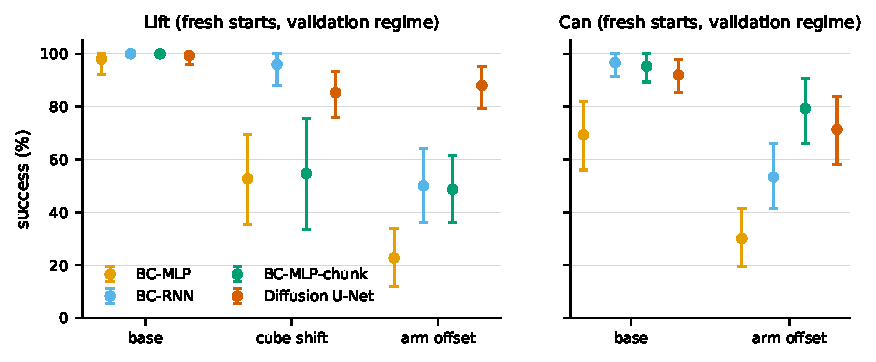
\includegraphics[width=\linewidth]{generated/figures/robustness.pdf}
\caption{Success per family on the base starts and under each perturbation (mean over seeds
with the \rf{proto.level}\,\% interval).}
\label{fig:robustness}
\end{figure}

\paragraph{Lift.} All four families succeed on at least \rf{rob.lift.bcmlp.base.succ}\,\% of
the base starts (Table~\ref{tab:robustness}, Figure~\ref{fig:robustness}). Under cube shift,
BC-MLP and BC-MLP-chunk fall to \rf{rob.lift.bcmlp.cube.succ} and
\rf{rob.lift.chunk.cube.succ}\,\%, diffusion to \rf{rob.lift.diff.cube.succ}\,\%, and BC-RNN
holds at \rf{rob.lift.bcrnn.cube.succ}\,\%. Under arm offset, diffusion keeps
\rf{rob.lift.diff.arm.succ}\,\%, against \rf{rob.lift.bcrnn.arm.succ}\,\% for BC-RNN,
\rf{rob.lift.chunk.arm.succ}\,\% for BC-MLP-chunk and \rf{rob.lift.bcmlp.arm.succ}\,\% for
BC-MLP. Diffusion exceeds BC-MLP-chunk on both sets (\rf{rob.lift.cube.diff-chunk.d} and
\rf{rob.lift.arm.diff-chunk.d}\,pp, both separated) and BC-RNN under arm offset
(\rf{rob.lift.arm.diff-bcrnn.d}\,pp, separated), while BC-RNN is ahead under cube shift
(diffusion minus BC-RNN \rf{rob.lift.cube.diff-bcrnn.d}\,pp, not separated).

\paragraph{Can.} The Lift pattern does not carry over. Under arm offset on Can, BC-MLP-chunk
keeps \rf{rob.can.chunk.arm.succ}\,\% and diffusion \rf{rob.can.diff.arm.succ}\,\%; their
difference (\rf{rob.can.arm.diff-chunk.d}\,pp [\rf{rob.can.arm.diff-chunk.lo},
\rf{rob.can.arm.diff-chunk.hi}]) is not separated. Diffusion does exceed BC-MLP
(\rf{rob.can.arm.diff-bcmlp.d}\,pp) and BC-RNN (\rf{rob.can.arm.diff-bcrnn.d}\,pp).

\paragraph{Reading H4.} Each Lift and Can analysis reports \rf{rob.lift.contrasts} and
\rf{rob.can.contrasts} differences and contrasts, unadjusted for multiplicity. The seed-level
sensitivity analysis (Table~\ref{tab:sens-rob} in the appendix) changes
\rf{sens.rob.changed} of \rf{sens.rob.n} robustness verdicts, all from separated to not
separated. Among them is diffusion's advantage over BC-MLP-chunk under Lift cube shift
([\rf{sens.rob.lift.cube.diff-chunk.lo}, \rf{sens.rob.lift.cube.diff-chunk.hi}]), whereas its
advantage under Lift arm offset stays separated under both methods. Two further
cautions apply. First, the diffusion sampler bounds every action to the range of the
training actions, while the BC heads are bounded only by the controller limits. In BC
episodes that fail under perturbation most motion actions lie outside that range, which
diffusion cannot do, so the between-family robustness gaps combine the generative model with
this output bound (Section~\ref{sec:limitations}). This is a correlation, not a mechanism:
the out-of-range actions start only after a grasp is missed, and BC-RNN rarely leaves the
range yet keeps only \rf{rob.lift.bcrnn.arm.succ}\,\% under arm offset. Second, the results hold
only for these two perturbations. We therefore read H4 as: on Lift, diffusion degrades least
under a large joint offset, and under cube shift BC-RNN degrades least, with diffusion not
separated from it; on Can, diffusion's drop under arm offset is not separated from the
chunked MLP's (\rf{rob.can.dd.arm.diff-chunk.d}\,pp [\rf{rob.can.dd.arm.diff-chunk.lo},
\rf{rob.can.dd.arm.diff-chunk.hi}]), whose point estimate is smaller.

\paragraph{Ablations.} Table~\ref{tab:ablations} reports the three preregistered diffusion
ablations on the robustness base starts. A1 evaluates the raw trained weights instead of
the EMA weights of the same checkpoints; A2 samples with DDPM over all \rf{diff.T} steps
instead of DDIM with \rf{diff.ddim}; A3 (Can only) trains a diffusion policy with one
observation instead of two (\rf{abl.A3.params.to1} instead of \rf{abl.A3.params.to2}
parameters, three new seeds, selected by the same rule). Checkpoints were selected with EMA
weights and DDIM-\rf{diff.ddim}, which favours the primary arm in A1 and A2, and all three
ablations share the primary arm's evaluations on the base starts, so they are not
independent of each other or of H4. None of the five differences is separated, by the
bootstrap or by the seed-level analysis. DDIM-\rf{diff.ddim} was not separated from DDPM over
all \rf{diff.T} steps, although both point estimates favour DDPM (\rf{abl.lift.A2.d} and
\rf{abl.can.A2.d}\,pp). No ablation of the action horizons ($T_p$, $T_a$) was run; the only comparison
that changes them is BC-MLP against BC-MLP-chunk, which also changes the observation window
and is not a declared comparison.

\begin{table}[t]
\centering\small
\caption{Diffusion ablations on the robustness base starts (\rf{proto.nseeds} seeds,
\rf{proto.nstates} starts each). A1 and A2 re-evaluate the selected checkpoints; A3 trains
separately. Primary: EMA weights, DDIM-10, $T_o = 2$.}
\label{tab:ablations}
\resizebox{\linewidth}{!}{% Generated by scripts/paper_assets.py (DECISIONS D-094). Do not edit.
% Sources (path sha256):
%   reports/session7/robustness/analysis.json 8cca66a8a8a8cecf0b734355167936e81983c821c625a23456523365409c9451
\begin{tabular}{llllll}
\toprule
 & Task & Arm $A$ (success \%) & Arm $B$ (success \%) & $A - B$ (pp) & Outcome \\
\midrule
A1 & Lift & primary 99.3 [96.0, 100.0] & trained weights 98.7 [95.3, 100.0] & \ensuremath{+}0.7 [\ensuremath{+}0.0, \ensuremath{+}2.7] & not separated \\
A1 & Can & primary 92.0 [84.7, 98.0] & trained weights 94.7 [88.7, 99.3] & \ensuremath{-}2.7 [\ensuremath{-}7.3, \ensuremath{+}0.7] & not separated \\
A2 & Lift & primary 99.3 [96.0, 100.0] & DDPM-100 100.0 [100.0, 100.0] & \ensuremath{-}0.7 [\ensuremath{-}4.0, \ensuremath{+}0.0] & not separated \\
A2 & Can & primary 92.0 [84.7, 98.0] & DDPM-100 95.3 [89.3, 100.0] & \ensuremath{-}3.3 [\ensuremath{-}10.0, \ensuremath{+}3.3] & not separated \\
A3 & Can & $T_o = 2$ 92.0 [84.7, 98.0] & $T_o = 1$ 94.0 [86.7, 99.3] & \ensuremath{-}2.0 [\ensuremath{-}8.7, \ensuremath{+}4.0] & not separated \\
\bottomrule
\end{tabular}
}
\end{table}

\paragraph{Failure modes.} Table~\ref{tab:taxonomy} and Figure~\ref{fig:taxonomy} classify
every held-out and Level~2 failure, and Table~\ref{tab:taxonomy-rob} every failure of the
robustness evaluations. Under Lift arm offset, BC-MLP's failures are mostly drifts
(\rf{rob.lift.bcmlp.arm.tax.no-grasp-drift} of its episodes), while diffusion has
\rf{rob.lift.diff.arm.tax.no-grasp-drift} drifts and fails mostly next to the cube
(\rf{rob.lift.diff.arm.tax.no-grasp-near}). On the Level~1 held-out starts, BC-MLP's Lift failures are mostly drifts away
from the cube without a grasp (\rf{l1.lift.bcmlp.tax.no-grasp-drift} of
\rf{l1.lift.n}$\times$\rf{proto.nseeds} episodes), while diffusion's few failures end near the
cube or after a drop. On Can, BC-MLP fails in several ways, most often by never closing the
gripper (\rf{l1.can.bcmlp.tax.gripper-never-closed} episodes). The point-cloud policy's
failures under cube shift are mostly misses near the cube (\rf{l2.pcdiff.cube.tax.no-grasp-near})
and drops (\rf{l2.pcdiff.cube.tax.dropped}), not drifts.

\begin{table}[t]
\centering\small
\caption{Failure taxonomy: episodes per category, summed over the three seeds (one run of
\rf{proto.nstates} episodes for the random baseline).}
\label{tab:taxonomy}
% Generated by scripts/paper_assets.py (DECISIONS D-094). Do not edit.
% Sources (path sha256):
%   reports/session7/results/results.json b8b097c38765c588711615917e3cfd5be6847e63083ddebe92f0f1488672408c
%   reports/session9/level2_results/results.json 1d33c975e49df907a6543b17e0cf36d047f7b5ce11aa69a355313e146c22571e
%   reports/session8/rgb_results/results.json 57663b81aafc70e9c1d850322b6bb1b894f7dad0d082976b1f546475a601390e
\begin{tabular}{lrrrrrrrr}
\toprule
Policy & \rotatebox{90}{success} & \rotatebox{90}{engineering error} & \rotatebox{90}{gripper never closed} & \rotatebox{90}{no grasp, drifted} & \rotatebox{90}{no grasp, near} & \rotatebox{90}{timeout holding} & \rotatebox{90}{in goal bin, not success} & \rotatebox{90}{dropped} \\
\midrule
\multicolumn{9}{l}{\emph{Level 1 held-out, Lift}} \\
BC-MLP & 136 & 0 & 0 & 12 & 0 & 0 & 0 & 2 \\
BC-RNN & 150 & 0 & 0 & 0 & 0 & 0 & 0 & 0 \\
BC-MLP-chunk & 147 & 0 & 0 & 3 & 0 & 0 & 0 & 0 \\
Diffusion U-Net & 146 & 0 & 0 & 0 & 3 & 0 & 0 & 1 \\
Random (uniform) & 0 & 0 & 0 & 38 & 9 & 0 & 0 & 3 \\
\multicolumn{9}{l}{\emph{Level 1 held-out, Can}} \\
BC-MLP & 115 & 0 & 11 & 8 & 4 & 3 & 2 & 7 \\
BC-RNN & 144 & 0 & 1 & 1 & 0 & 0 & 3 & 1 \\
BC-MLP-chunk & 144 & 0 & 1 & 0 & 4 & 0 & 1 & 0 \\
Diffusion U-Net & 143 & 0 & 0 & 2 & 0 & 0 & 3 & 2 \\
Random (uniform) & 0 & 0 & 0 & 44 & 6 & 0 & 0 & 0 \\
\multicolumn{9}{l}{\emph{RGB study held-out, Lift}} \\
Visual diffusion & 150 & 0 & 0 & 0 & 0 & 0 & 0 & 0 \\
Visual BC-chunk & 149 & 0 & 0 & 0 & 1 & 0 & 0 & 0 \\
\multicolumn{9}{l}{\emph{Level 2, Lift}} \\
Point-cloud diffusion, held-out & 150 & 0 & 0 & 0 & 0 & 0 & 0 & 0 \\
Point-cloud diffusion, cube shift & 85 & 0 & 0 & 4 & 45 & 0 & 0 & 16 \\
Point-cloud diffusion, base & 150 & 0 & 0 & 0 & 0 & 0 & 0 & 0 \\
Visual diffusion, cube shift & 147 & 0 & 0 & 0 & 3 & 0 & 0 & 0 \\
Visual diffusion, base & 150 & 0 & 0 & 0 & 0 & 0 & 0 & 0 \\
\bottomrule
\end{tabular}

\end{table}

\begin{table}[t]
\centering\small
\caption{Failure taxonomy of the robustness evaluations (validation regime), summed over the
three seeds.}
\label{tab:taxonomy-rob}
% Generated by scripts/paper_assets.py (DECISIONS D-094). Do not edit.
% Sources (path sha256):
%   reports/session7/robustness/analysis.json 8cca66a8a8a8cecf0b734355167936e81983c821c625a23456523365409c9451
\begin{tabular}{lrrrrrrrr}
\toprule
Policy & \rotatebox{90}{success} & \rotatebox{90}{engineering error} & \rotatebox{90}{gripper never closed} & \rotatebox{90}{no grasp, drifted} & \rotatebox{90}{no grasp, near} & \rotatebox{90}{timeout holding} & \rotatebox{90}{in goal bin, not success} & \rotatebox{90}{dropped} \\
\midrule
\multicolumn{9}{l}{\emph{Lift, base}} \\
BC-MLP & 147 & 0 & 0 & 3 & 0 & 0 & 0 & 0 \\
BC-RNN & 150 & 0 & 0 & 0 & 0 & 0 & 0 & 0 \\
BC-MLP-chunk & 150 & 0 & 0 & 0 & 0 & 0 & 0 & 0 \\
Diffusion U-Net & 149 & 0 & 0 & 0 & 0 & 0 & 0 & 1 \\
\multicolumn{9}{l}{\emph{Lift, cube shift}} \\
BC-MLP & 79 & 0 & 5 & 57 & 1 & 0 & 0 & 8 \\
BC-RNN & 144 & 0 & 0 & 4 & 0 & 0 & 0 & 2 \\
BC-MLP-chunk & 82 & 0 & 0 & 49 & 7 & 0 & 0 & 12 \\
Diffusion U-Net & 128 & 0 & 0 & 1 & 15 & 0 & 0 & 6 \\
\multicolumn{9}{l}{\emph{Lift, arm offset}} \\
BC-MLP & 34 & 0 & 2 & 104 & 6 & 0 & 0 & 4 \\
BC-RNN & 75 & 0 & 7 & 57 & 5 & 0 & 0 & 6 \\
BC-MLP-chunk & 73 & 0 & 0 & 67 & 3 & 0 & 0 & 7 \\
Diffusion U-Net & 132 & 0 & 0 & 0 & 12 & 1 & 0 & 5 \\
\multicolumn{9}{l}{\emph{Can, base}} \\
BC-MLP & 104 & 0 & 16 & 9 & 4 & 2 & 8 & 7 \\
BC-RNN & 145 & 0 & 1 & 1 & 0 & 0 & 2 & 1 \\
BC-MLP-chunk & 143 & 0 & 2 & 1 & 1 & 0 & 1 & 2 \\
Diffusion U-Net & 138 & 0 & 0 & 0 & 2 & 1 & 4 & 5 \\
\multicolumn{9}{l}{\emph{Can, arm offset}} \\
BC-MLP & 45 & 0 & 17 & 60 & 13 & 0 & 6 & 9 \\
BC-RNN & 80 & 0 & 6 & 43 & 2 & 6 & 4 & 9 \\
BC-MLP-chunk & 119 & 0 & 5 & 8 & 9 & 0 & 3 & 6 \\
Diffusion U-Net & 107 & 0 & 8 & 7 & 8 & 0 & 4 & 16 \\
\bottomrule
\end{tabular}

\end{table}

\begin{figure}[t]
\centering
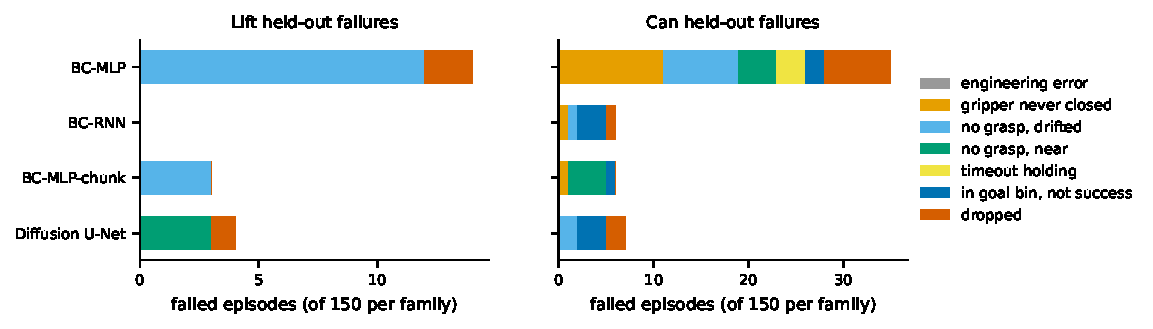
\includegraphics[width=\linewidth]{generated/figures/taxonomy.pdf}
\caption{Failure categories of the Level~1 held-out episodes per family (successes omitted).}
\label{fig:taxonomy}
\end{figure}
